 \documentclass[12pt,letterpaper]{article}
\usepackage[margin=1.0in]{geometry}
\usepackage[utf8]{inputenc}
\usepackage{cite}
\usepackage{amsmath}
\usepackage{amsfonts}
\usepackage{amssymb}
\usepackage{makeidx}
\usepackage{graphicx}
\usepackage{hyperref}
\setlength\parindent{0pt}

\author{STUDENT NAME}
\title{HW: Mandelbrot Fractal Programming in MatLab}

\begin{document}

\maketitle

\section{Objective}
The purpose of this homework is to give the student a thorough exercise in MatLab programming, and en passe appreciate the concept of mathematical complexity.\\ 

\section{Introduction}
Before fractal geometry was discovered by \href{https://en.wikipedia.org/wiki/Benoit_Mandelbrot}{Benoit Mandelbrot}, we only had Euclidian geometry which cannot describe "natural" objects such as mountains, clouds, trees, plants, lungs, artery systems etc. Since agricultural engineering is about connecting living objects to technology, it is only natural (pun intended) to discuss fractals.\\

\href{http://en.wikipedia.org/wiki/Benoit_Mandelbrot}{Benoit Mandelbrot} is credited with being the first person to visualize mathematical complexity in a spectacular way. The idea is to take a non-linear equation, and iterate it, meaning that you give it a starting value and then calculate a new value by entering this starting value into the equation. Then you take the result of the equation, put it back in and calculate a new value. You keep doing this and check if the value eventually goes to infinity (or out of a preset bound) or if it stays within the bound. You also keep track of how many iterations it took for the value to go out of the bound, you use that to assign a color.

To calculate the Mandelbrot fractal, we need to use the complex plane that runs from $[-2.5, 1.5]$ on the real axis and $[-1.5,1.5]$ in the imaginary axis. 

\begin{figure}
\centering
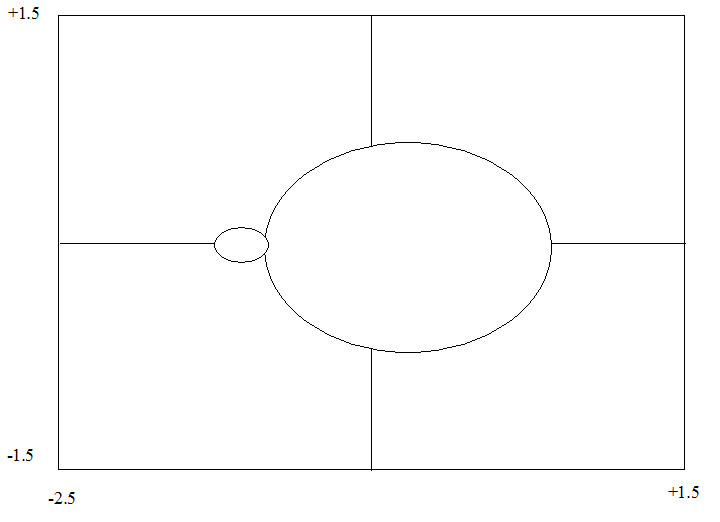
\includegraphics[width=0.7\linewidth]{HW_MandelbrotFractalCoordinates}
\caption{Coordinate frame of the Mandelbrot fractal running from x = [-2.5, 1.5] and y = [-1.5, 1.5]. We split the axes into pixels to generate a fractal of say 4000 * 3000 pixels. Each pixel now represents a complex number, from which we will evaluate whether it is bounded or not under iteration using the logistics equation given.}
\label{fig:HW_MandelbrotFractalCoordinates}
\end{figure}

The equation we are going to use is a logistics equation:

\begin{equation}\label{Eqn:HW_Mandelbrot1}
z(n+1) = z(n)^2 + c
\end{equation}

where $z$ and $c$ are complex numbers, and $n$ indicates the iteration (look at $z(n)$ as the previous value of $z(n+1)$). For the programming it is easiest to split our complex number into a real and imaginary part (although you don't have to, MatLab can deal with complex numbers quite well). However, we would have to use "r" for real and "j" for imaginary, in our case it is much easier to look at the x-axis as the real axis and the y-axis as the imaginary axis. This makes the notation much more in line with a program that would use an x and y axis. Therefore we'll define $z_r = z_x$ and $z_j = z_y$. Our complex number $z$ now becomes:



\begin{equation}\label{Eqn:HW_Mandelbrot2}
z = z_x + j z_y
\end{equation}

If we substitute this form into the logistics equation we get:

\begin{equation}\label{Eqn:HW_Mandelbrot3}
z(n+1) = z_x(n+1) + j z_y(n+1) = \left[ z_x(n) + j z_y(n) \right]^2 + c_x + c_y 
\end{equation}

Evaluating the square gives:

\begin{equation}\label{Eqn:HW_Mandelbrot54}
z(n+1) = z_x(n+1) + j z_y(n+1) = z_x(n)^2 + 2 j z_x(n) z_y(n) - z_j(n)^2 + c_x + c_y 
\end{equation}

Splitting the real and imaginary parts gives:

\begin{equation}\label{Eqn:HW_Mandelbrot5}
z_x(n+1) = z_x(n)^2 - z_y(n)^2 +c_x
\end{equation}

and:

\begin{equation}\label{Eqn:HW_Mandelbrot6}
z_y(n+1) = 2z_x(n) z_y(n) + c_y
\end{equation}

The constant $c$ is quite important. If you set this factor to a constant number in the range as shown in Figure \ref{fig:HW_MandelbrotFractalCoordinates}, then you get what is known as a Julia Fractal (after \href{http://en.wikipedia.org/wiki/Gaston_Julia}{Gaston Julia} , a French mathematician). However, if you set the constant $c$ equal to the coordinate of the pixel under calculation, then you get the Mandelbrot fractal, which is our aim here.\\

\section{Program structure}
The variables as shown in Equations \ref{Eqn:HW_Mandelbrot5} and \ref{Eqn:HW_Mandelbrot6} look good in a report, but MatLab cannot read them as such (for instance MatLab does not regard z\_n+1 a variable). Therefore we need some representatives. Let's assign z\_x\_new to $z_x(n+1)$ and z\_x\_old to $z_x(n)$ and z\_y\_new to $z_y(n+1)$ and z\_y\_old to $z_y(n)$. We will write x\_coor for $c_x$ and y\_coor for $c_y$.\\

The program has three major sections that are executed in sequence being 1) Initialization, 2) Calculation and 3) Output (a graph). In the intialization section, you set constants and give them logical names. 
Give a value to MaxIterations to say 100. This variable sets a limit to the maximum number of iterations that we will do before we quit. The boundaries of our fractal are x\_min = -2.5 and x\_max = 1.5, y\_min = -1.5, y\_max = 1.5. The program needs to begin by entering the boundary coordinates and a step size to calculate the coordinates of our pixels. If we want a 400 * 300 image, then we the x-stepsize would be $\dfrac{4}{400} = 0.01$ and the y-stepsize would be $\dfrac{3}{300} = 0.01$.\\

Now we need to create an "empty" image that we can use to write values to (you'll see later what values). The easiest trick is to fill that "empty" image with MaxIterations, it just looks good.\\

Now we have to run through all rows, and all columns to address each pixel. We start with the coordinate of the pixel and then iterate the real and imaginary parts of the pixel using equations \ref{Eqn:HW_Mandelbrot5} and \ref{Eqn:HW_Mandelbrot6}. You iterate these calculations, until the absolute value $A = \left|  z(n+1) \right| = \sqrt{z_r(n+1)^2 + z_j(n+1)^2} $ becomes larger than 2 OR we exceed a preset number of iterations. If the absolute value of the trajectory goes out of the bound (2) then we write the number of iterations as the pixel value in our current coordinate. This method shows the "depth" of the Mandelbrot fractal structure. We also need to set a limit to the number of iterations to avoid getting into an infinite loop. If a trajectory has not gone out of the bound (2) within say 100 iterations, we conclude that it is bounded and do nothing, at that point the pixel keeps the value it was assigned before the calculations. 

Now we need to go through the whole image starting at the bottom left (x\_min, y\_min) and work our way through every pixel row by row. For this we need two nested loops. 

Inside the hot loop, we need to calculate the absolute value $\left|  z(n+1) \right|$ and keep track of for how many iterations it stays withing the limit of 2. Some pixels will stay bounded forever so we need to set a limit to the maximum number of iterations to prevent getting stuck in an infinite loop. Finally we plot the Fractal image using imagesc (which scales it properly).\\

The complete process is shown in a Nassi-Shneiderman diagram in Figure \ref{fig:MandelbrotNSDiagram}. Figure \ref{fig:HW_Mandelbrot1} shows the Mandelbrot fractal. \\

\begin{figure}
\centering
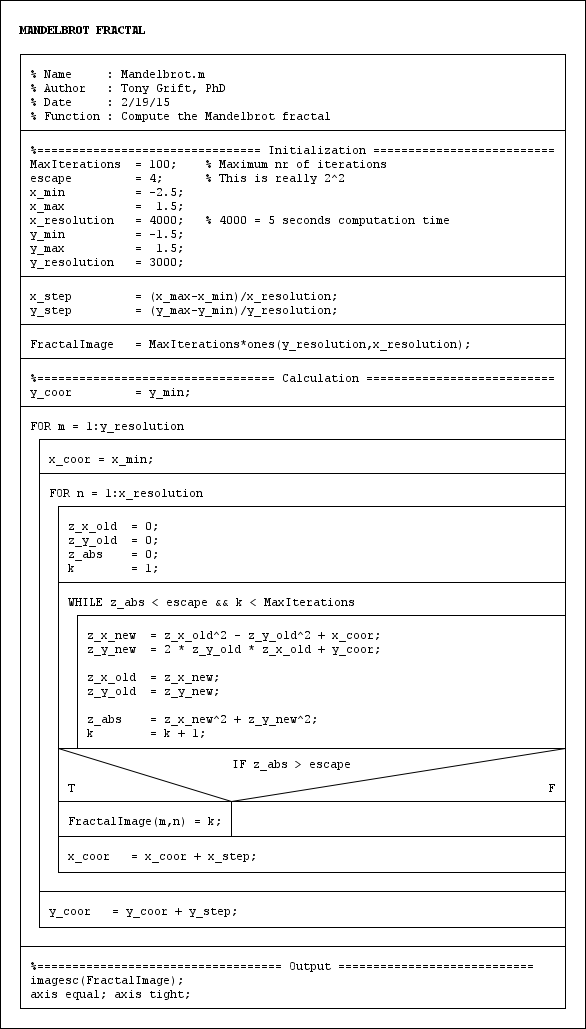
\includegraphics[width=0.75\linewidth]{MandelbrotNSDiagram}
\caption{Here a \href{http://en.wikipedia.org/wiki/Nassi-Shneiderman_diagram}{Nassi-Shneiderman diagram}  is shown which contains all actions that we need to do to calculate the Mandelbrot Fractal. Notice that the NS diagram has special blocks for a statement, FOR loop, While loop etc.}
\label{fig:MandelbrotNSDiagram}
\end{figure}


\begin{figure}
\centering
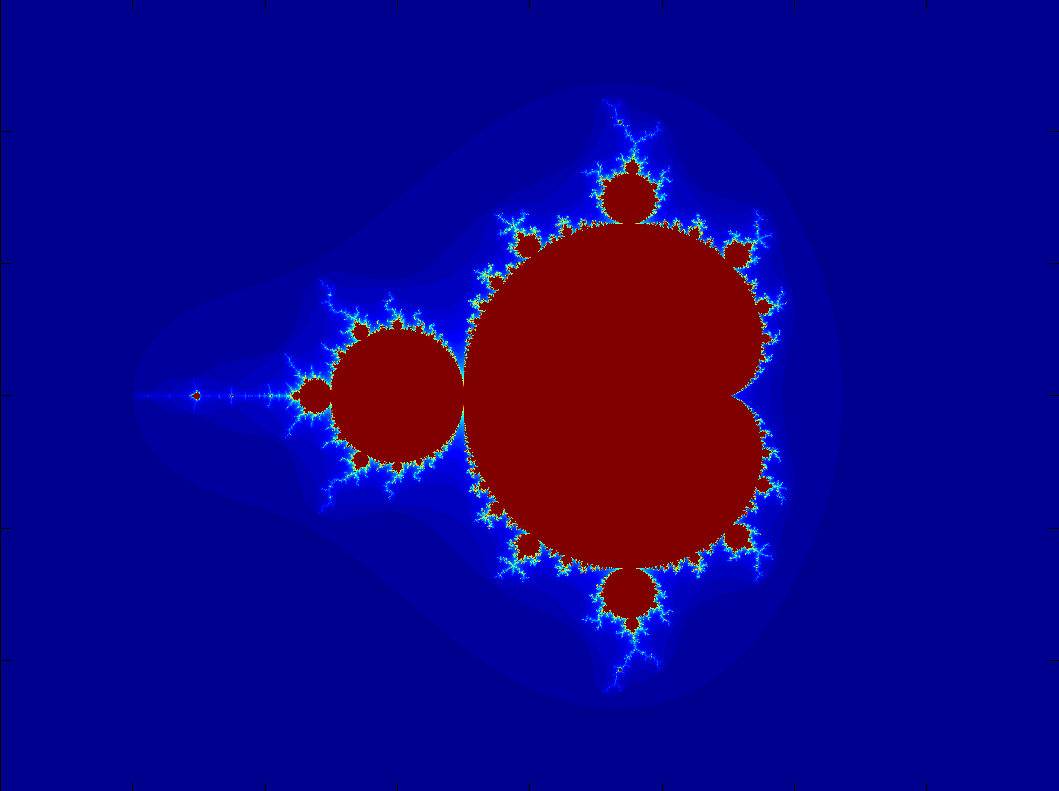
\includegraphics[width=1\linewidth]{HW_Mandelbrot1}
\caption{Mandelbrot Fractal, the pinnacle of mathematical self-similarity. The areas inside the circle and the "apple" are bounded, that means within 100 iterations, the absolute value of their z's do not exceed the escape value 2. All other pixels eventually exceed the escape value, but some do that faster than others, which is indicated by the coloring. When studying the Mandelbrot fractal, you need to think about how it is possible that the simplest of equations can yield such amazing depth and detail. As Mandelbrot himself used to say: "Think not of what you see, but what it took to produce what you see".}
\label{fig:HW_Mandelbrot1}
\end{figure}

The first thing that should strike you (I hope) is that there is an overwhelming amount of detail, self-similarity (\underline{the} feature that characterizes a fractal) and unique areas in the Mandelbrot fractal. The most baffling thing is that all this emerges from iterating a very simple equation! The intuitive idea that a complex object needs a complex underlying mechanism is obviously false! For instance when you see the pattern of the coat of a cat (see Figure \ref{fig:MaineCoon_SolidBlackCat}), you would imagine that many genes may be involved to produce this kind of complexity. It turns out that is not the case, only a handful of genes make up the difference between a solid colored cat and a Maine coon (note the M on this cat's forehead).\\

\begin{figure}
\centering
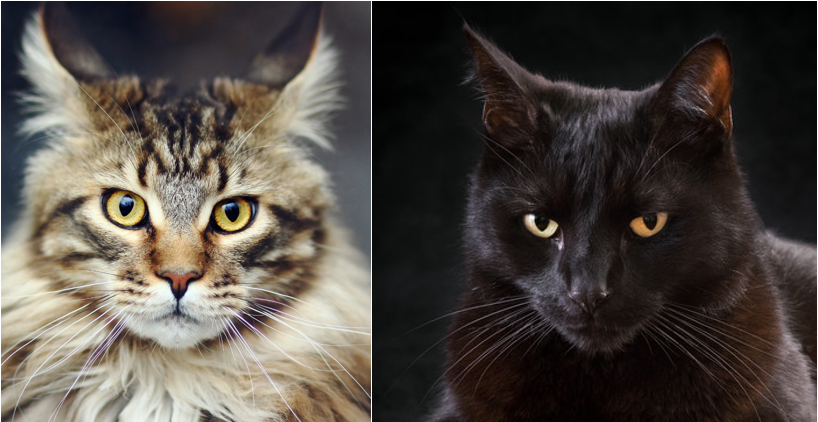
\includegraphics[width=1\linewidth]{MaineCoon_SolidBlackCat}
\caption{Compare a Maine Coon cat (left) with elaborate striping to a solid black cat. One would expect that the striping of the Maine Coon (notice the M on this cat's forehead) would require a large number of genes. That is not the case, even a small number of genes can give rise to enormous differences in phenotype. Complexity can arise from very simple rules.}
\label{fig:MaineCoon_SolidBlackCat}
\end{figure}

Q1: Give the name of the fractal shown in Figure \ref{fig:HW_Q1Fractal} (The answer can be found in the Nova documentary "Hunting the hidden dimension").

\begin{figure}
\centering
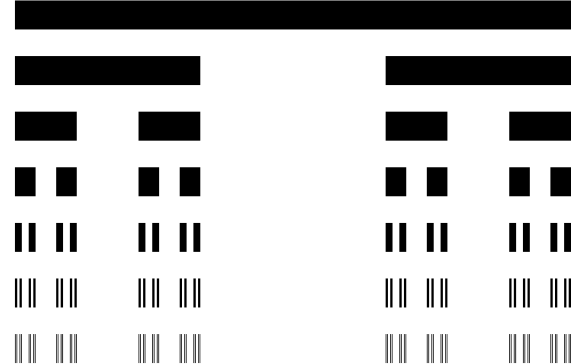
\includegraphics[width=0.6\linewidth]{HW_Q1Fractal}
\caption{Elementary Fractal. You need to find its name by watching the NOVA video "Hunting the hidden dimension".}
\label{fig:HW_Q1Fractal}
\end{figure}

A1:


\end{document}